\documentclass{math201}
\usepackage{hyperref}
\usepackage{bookmark}
\usepackage{minted}

% =============================================
% Part 0 信息
% =============================================

\mathsetup{
  % 学生姓名
  student = {某同学},
  % 学号
  student-id = {2021xxxx},
  % 院系
  experiment = {实验一 GPIO点亮LED},
  % 专业年级
  discipline = {集成电路设计与集成系统},
  % 日期
  date = {\today},
}

\begin{document}

% =============================================
% Part 1  封面
% =============================================

\makecover

% =============================================
% Part 2 主文档
% =============================================

\section{实验要求}

\begin{enumerate}
  \item 运行例程\textbf{实验1 GPIO点亮LED},观察实验现象
  \item 看懂源程序
  \item 修改源程序,使用3种方法实现交通信号灯循环3次,红灯,黄灯,绿灯,黄灯……
  \item 增加:在上面第2条中增加,黄灯亮的同时蜂鸣器响
  \item 完成实验报告,把修改的程序截图、实验现象截图或者图片整理到报告中。
\end{enumerate}

\section{实验内容及结果}

\subsection{编写代码}

具体来说,可以通过以下几种方式控制 LED 的亮灭:

\begin{enumerate}
  \item 带参数的宏,可以像内联函数一样使用 \texttt{LED1(a)}、\texttt{LED2(a)}、\texttt{LED3(a)}
  \item 直接操作寄存器的方法控制IO: \texttt{digitalHi(p, i)}、\texttt{digitalLo(p, i)}、\texttt{digitalToggle(p, i)}
  \item 定义控制IO的宏: \texttt{LED1\_TOGGLE}、\texttt{LED1\_OFF}、\texttt{LED1\_ON}
\end{enumerate}

下面是实际可用的代码:

\inputminted[
    frame=lines,
    framesep=2mm,
    baselinestretch=1.2,
    fontsize=\small,
    linenos
]{C++}{code/main.c}

\subsection{下载运行}

使用 \texttt{FlyMCU.exe} 下载程序到 STM32 开发版上,观察实验现象。

\subsection{实验现象}

\begin{figure}[H]
  \centering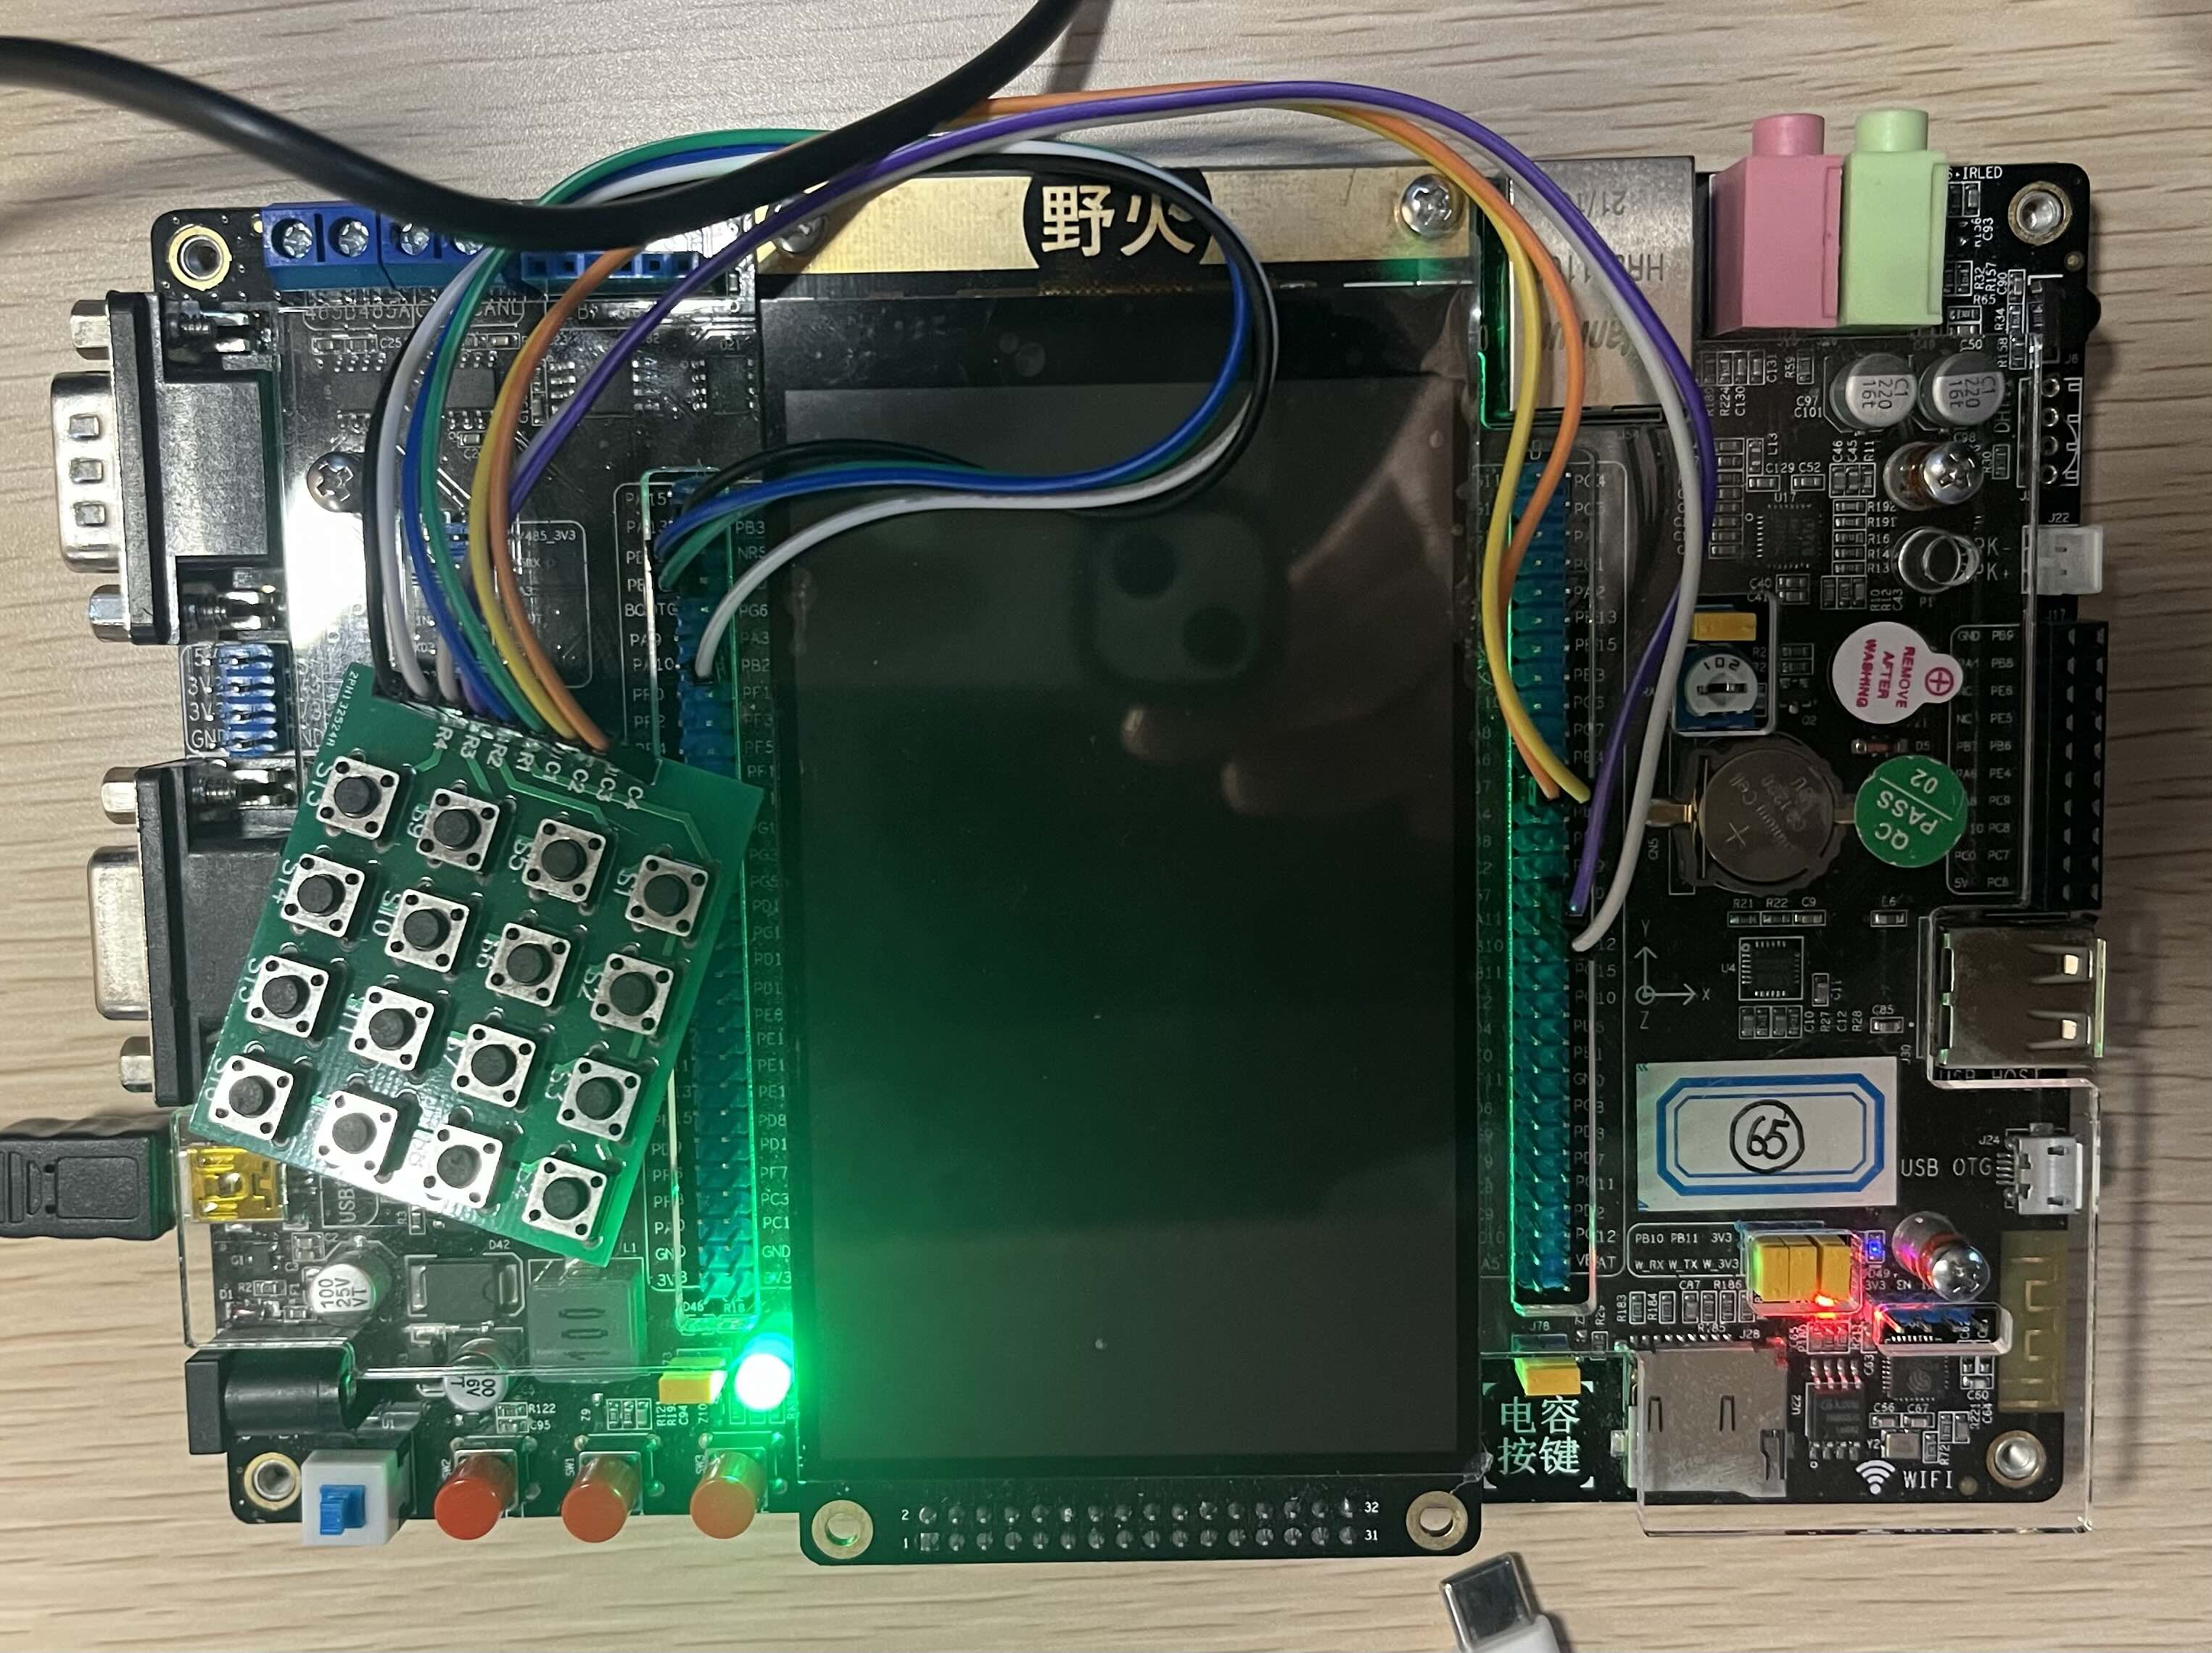
\includegraphics[width=0.6\linewidth]{led_green.jpg}
  \caption{绿灯亮}      
\end{figure}

\begin{figure}[H]
  \centering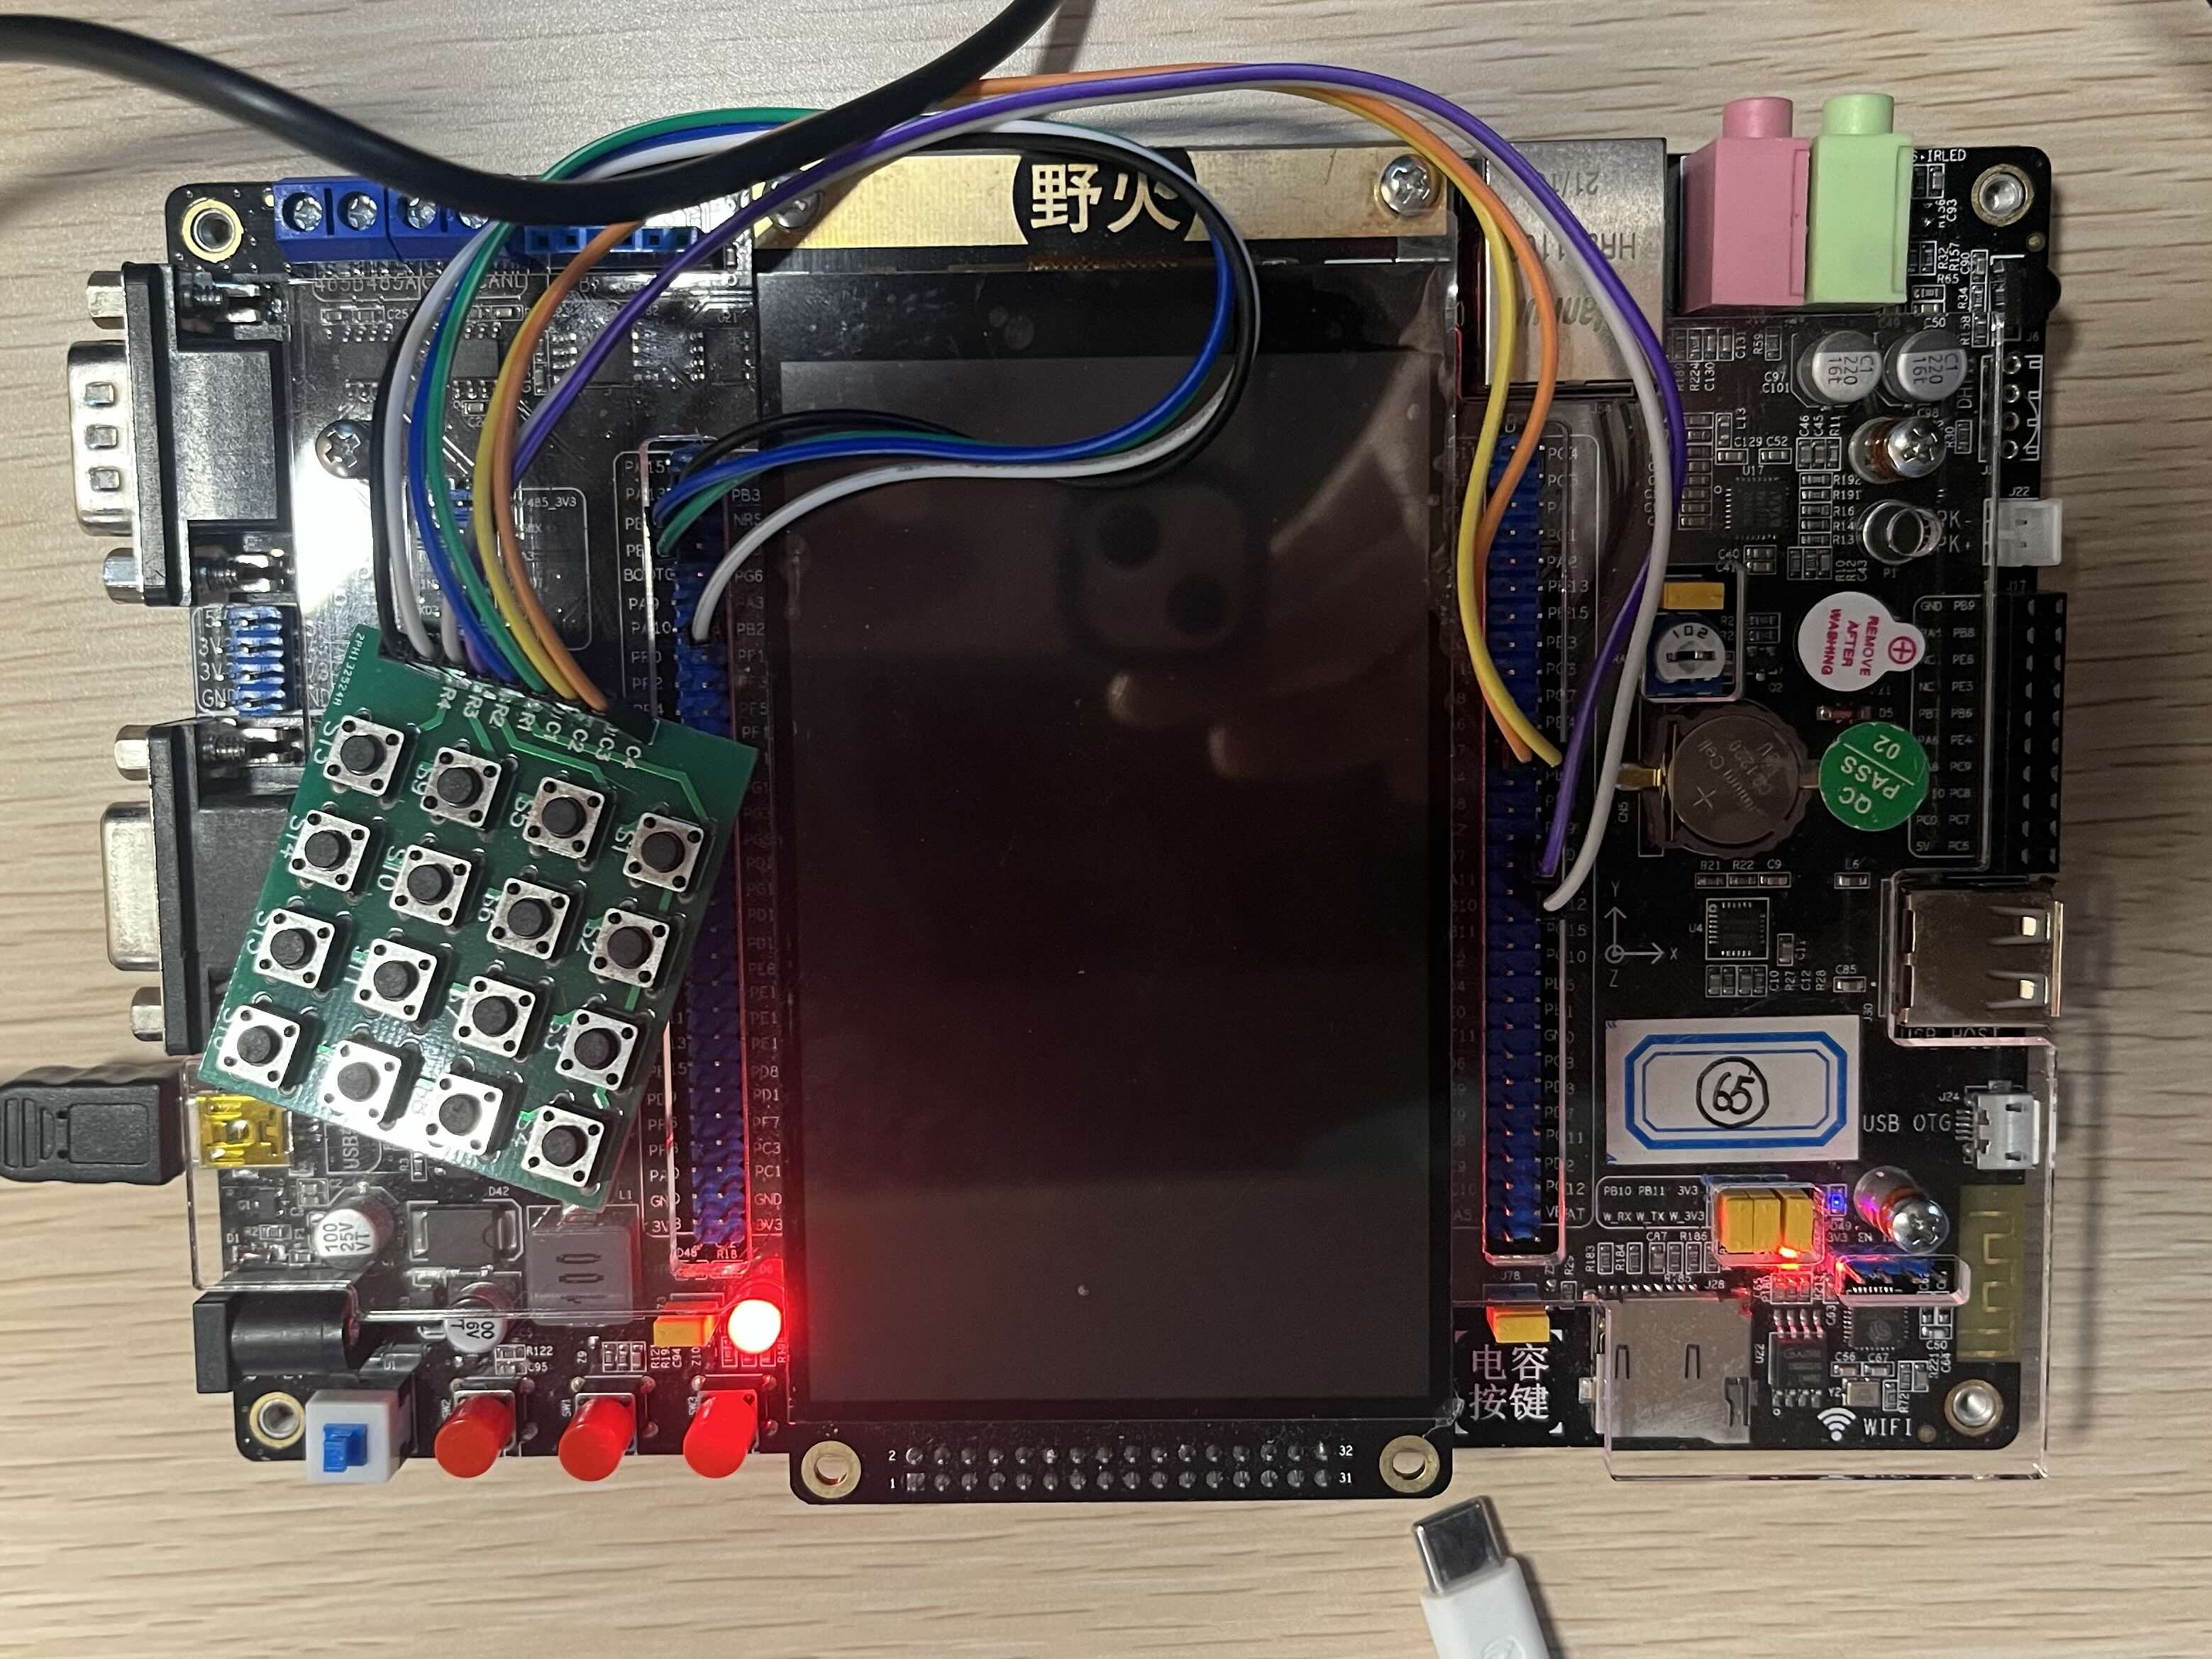
\includegraphics[width=0.6\linewidth]{led_red.jpg}
  \caption{红灯亮}
\end{figure}

\section{实验小结}

通过这次实验,我掌握了STM32开发板LED的控制方法,并学会了使用宏定义简化代码,以及如何修改源程序实现特定的功能。

这次实验让我对STM32开发板有了更深入的了解,也提高了我的编程能力。在实验过程中,我遇到了一些问题,如何实现循环等。通过查阅资料和上课听讲,我最终解决了这些问题。这次实验让我意识到,学习编程需要不断练习和思考,遇到问题要积极寻求解决办法。

\end{document}
